% !TeX root = ../Thesis.tex

\chapter{Neues Konzept} \label{ch:NewMethods}
\section{Überblick}
Das nachfolgende Kapitel beschreibt und diskutiert im Detail das angewandte Konzept der vorliegenden Thesis. 
Es behandelt die selbstentwickelten Beiträge zu den Methoden sowie die vorliegenden dreidimensionalen Bildstapel der Myotuben-Zellkulturen.
Auf die in Abschnitt \ref{sec:daten} beschriebenen Daten werden die eingeführten Methoden angewandt, um deren Effektivität zu demonstrieren.
In Abschnitt \ref{sec:Kriterien} wird ein neues Bewertungskriterium für 3D-Instanzsegmentierungsmodelle eingeführt.
Es bewertet Modelle im Hinblick auf ihre Eignung, interpretierbare Merkmale von Nuclei unverändert zu extrahieren.
Abschnitt \ref{sec:MethodsClassifier} führt Methoden zur Klassifikation von 3D-Daten ein.
Diese Methoden passen den Klassifikator an verschiedene Eigenschaften eines Datensatzes an.\\[0.5\baselineskip]
Die gesamte Methodik wird in einer modularen Anwendung umgesetzt, die 3D-Daten als Eingabe annimmt und interpretierbare Eigenschaften, wie die Verteilung der Klassen und das Volumen der anwesenden Nuclei, ausgibt.
Diese Anwendung wird hier als 3D-Zelldaten-Pipeline bezeichnet.
Abb. \ref{fig:graph_abstract} bietet einen Überblick über die Methodik.
Die Anwendung kann regulär angewandt (Inferenz) oder optimiert werden (Optimierung).
Zur Optimierung werden die 3D-Daten einem Ablauf für den Vergleich der Segmentierungsmodelle oder der Klassifikatormethoden zur Verfügung gestellt.
Zuerst wird das neu eingeführte Bewertungskriterium für Segmentierungsmodelle \acf{ipq} für verschiedene Modelle berechnet (siehe Kapitel \ref{sec:Kriterien}).
Dieses Bewertungskriterium quantifiziert die Eignung der Segmentierungsmodelle zur Extraktion der gewünschten Zellkerneigenschaften.
Mithilfe der \ac{ipq}-Werte wird das beste Segmentierungsmodell für die Anwendung gewählt.
Die Architektur und Parameter des optimalen Modells werden in den Inferenzablauf eingesetzt.\\[0.5\baselineskip]
Um die Klassifikatormethoden zu optimieren, werden die 3D-Daten und die extrahierten Segmente in die neu entwickelte Labeling-App eingegeben.
Die Labeling-App ermöglicht die zeiteffiziente Annotation von Nuclei, indem relevante Bildausschnitte automatisch anhand der Segmente extrahiert werden.
Mit den erstellten Annotationen und den 3D-Daten werden iterativ verschiedene Klassifikatoren trainiert.
Diese Klassifikatoren ergeben sich aus Kombinationen der verfügbaren Klassifikatormethoden.
Die Klassifikatormethoden werden in Kapitel \ref{sec:MethodsClassifier} beschrieben und umfassen 1. Encoder-Architekturen, 2. Klassifikations-Kopf-Architekturen, 3. Vorverarbeitungsmethoden und 4. Vortrainingsmethoden.
Unter den Methoden sind sowohl etablierte als auch neu entwickelte Ansätze.
Anhand der Genauigkeit der trainierten Klassifikatoren auf einem separaten Validierungsanteil des Datensatzes werden die Methoden verglichen und eine optimale Konfiguration ausgegeben.
Die Architektur und Parameter dieser Konfiguration werden dann in den Inferenzablauf der Anwendung eingesetzt.\\[0.5\baselineskip]
Am Ende des Ablaufs werden die klassifizierten Segmente verwendet, um verschiedene Grafiken zu erzeugen, die interpretierbare Eigenschaften visualisieren.
\begin{figure}[h]
  \centering
  \includegraphics[width=0.99\linewidth]{Figures/graphAbstract_flowchart.pdf}
  \caption{Methodik der vorliegenden Arbeit.
  Die Anwendung kann regulär angewandt (Inferenz) oder optimiert werden (Optimierung).
  Die Optimierung ist zweiteilig.
  Zur Optimierung der Segmentierungsmodelle wird das neu entwickelte \acf{ipq}-Bewertungskriterium eingesetzt.
  Für den Klassifikator werden Kombinationen verschiedener Encoder, Klassifikations-Köpfe, Vorverarbeitungsmethoden und Vortrainingsmethoden iterativ trainiert und verglichen. 
  }
  \label{fig:graph_abstract}
\end{figure}
\noindent

\section{Daten}\label{sec:daten}
Die zugrunde liegenden Bilddaten der vorliegenden Arbeit stammen aus in-vitro-Kulturen von Myotuben, die aus humanen induzierten pluripotenten Stammzellen (hiPSC) differenziert wurden. 
Diese Zellen wurden nach dem in Couturier et al. \cite{Couturier2024} beschriebenen Protokoll hergestellt und anschließend mittels Immunfluoreszenzfärbung markiert. 
Von den Zellen wurden 3D-Bildstapel mit voxelbasierten Intensitätswerten, die jeweils einem Fluoreszenzkanal zugeordnet sind, mit einem Konfokalmikroskop aufgenommen.
Die Kulturen enthalten Myotuben und deren Nuclei in fünf Fluoreszenzkanälen, die entsprechend mit fünf unterschiedlichen Fluoreszenzmarkern angefärbt wurden:
\begin{itemize}
  \item DAPI (Nuclei),
  \item $\alpha$-Actinin (sarcomerisches Strukturprotein),
  \item Dystrophin (Membran-assoziiertes Muskelprotein),
  \item Synaptophysin (präsynaptisches Vesikelprotein),
  \item $\alpha$-Bungarotoxin (Bindung an nikotinische Acetylcholinrezeptoren, nAChR) und
  \item S100$\beta$ (Schwannzellmarker).
\end{itemize}
Jeder dieser Marker färbt einen anderen Zellbestandteil an, sodass unter dem Mikroskop sichtbar ist, wo sich Kerne, Muskelfasern und synaptische Strukturen befinden.
Die Bildaufnahme erfolgte mit einem Leica TCS SP8 Konfokalmikroskop, unter Verwendung von 405-nm-, 488-nm-, 561-nm- und 633-nm-Lasern und einem 20x-Objektiv. 
Je Kanal ergibt sich eine räumliche Auflösung von 1024 x 1024 Pixeln mit 568 nm pro Pixel.
Die Anzahl der Z-Schichten beträgt 24 bis 64.
Die Proben wurden in Matrigel eingebettet und unter physiologisch relevanten Kulturbedingungen (37 °C, 5\% CO₂) im maturierenden Medium kultiviert, das u. a. Wachstums- und Differenzierungsfaktoren wie BDNF, GDNF, IGF-1, CHIR99021, DMH1, SB431542, Retinsäure und Purmorphamin enthielt.
Das resultierende Material stellt ein menschliches in-vitro-Modell der neuromuskulären Verbindung dar.
Abb. \ref{fig:channel_examples} zeigt exemplarisch je eine 2D-Schicht von einem der Marker-Kanäle.
\begin{figure}[H]
  \centering
  \includegraphics[width=0.9\linewidth]{Figures/channel_examples.pdf}
  \caption{Beispiele von 2D-Schnitten der verfügbaren Färbungen der vorliegenden 3D-Bildstapel.
  }
  \label{fig:channel_examples}
\end{figure}
\noindent
Die eingeführten Methoden werden als Experiment auf diese Daten angewandt, sie sind aber explizit entworfen, um Anpassungen an neue Datensätze nahtlos zu ermöglichen.
Alle Experimente auf diesen Daten dienen der vorliegenden Arbeit als Fallstudie, um die Effektivität der vorgestellten Methoden zu demonstrieren.
\section{Neues Kriterium: Injektive Panoptische Qualität}\label{sec:Kriterien}
Zur Wahl des Segmentierungsmodells wird das neue Bewertungskriterium \acf{ipq} eingeführt.
Es besteht aus drei Faktoren, die jeweils eine Fehlerart bei Instanzsegmentierungsmasken prüfen.
\begin{figure}[h]
  \centering
  \includegraphics[width=0.99\linewidth]{Figures/IPQ_horizontal.pdf}
  \caption{\ac{ipq} Visualisierung - Das Ablaufdiagramm stellt den Prozess dar, durch den das Segmentierungsmodell gewählt wird, das für die Anwendung der vorliegenden Arbeit eingesetzt wird. 
  Ein peer-reviewed Benchmark-Datensatz aus dreidimensionalen Bildern (1) von diversen Zellkulturen mit den dazugehörigen Annotationen wird links eingegeben. 
  Das zu bewertende Segmentierungsmodell (2) führt für die Bilder des Benchmarks eine Inferenz durch, um Segmentierungsmasken (3) bereitzustellen. 
  Die entstehenden Masken werden anschließend zur Berechnung der neu eingeführten \ac{ipq} (siehe Kapitel \ref{sec:Kriterien}) eingesetzt. 
  Der Ablauf der Bewertung ist in drei Phasen gegliedert.
  Aus jeder Maske werden zuerst die einzelnen Fragmente extrahiert, die sich mit einer einzelnen Instanz der Annotation überlagern (4).
  Außerdem wird ein Fehlerbild durch Berechnung der \acf{iou} hergestellt, hier als logische XOR-Fläche der Maske und der Annotation als Platzhalter dargestellt (5).
  Zuletzt wird ein Zuweisungsbild erstellt, das die \acp{tp}, \acp{fp} und \acp{fn} festhält (6).
  Aus diesen drei Teilen wird jeweils ein Faktor zur Berechnung der \ac{ipq} gebildet.
  Durch Vergleiche der Ergebnisse verschiedener Modelle lässt sich dann das optimale Segmentierungsmodell für die Anwendung wählen.}
  \label{fig:ipq}
\end{figure}
\noindent
Als Datensatz wird aus den in Kapitel \ref{sec:bench} vorgestellten Benchmarks der S\_BIAD1518-Datensatz \cite{Kromp2020_Dataset, chen20223_Dataset} verwendet, da dieser nicht in den Trainingsdaten eines zu testenden Segmentierungsmodells vorkommt.
Der Datensatz verfügt über manuelle Annotationen für Instanzsegmentierungsmasken und ist durch synthetisch generierte Daten und Masken erweitert.
Im Gegensatz zu selbstentwickelten synthetischen Daten weicht die Bilddomäne dieses Benchmarks zwar stärker von der Domäne der Zieldaten ab, aber dafür sind die Daten an eine Veröffentlichung mit standardisiertem Peer-Review-Prozess gebunden.\\ [0.5\baselineskip]
Die Aufgabe des Bewertungskriteriums ist es, zu quantifizieren, wie gut sich eine vorliegende Instanzsegmentierung eignet, um reale Eigenschaften einer Aufnahme, wie die Zellkernanzahl, die Größe der Zellkerne und die lokale Zellkerndichte auszuwerten. 
Das neu entwickelte Kriterium ist eine Erweiterung der \ac{pq} \cite{kirillov2019PQ}. 
Durch die \ac{pq} wird die \ac{iou} für individuelle Instanzen bewertet und es werden \ac{fp} sowie \ac{fn} Detektionen bestraft. 
Zusätzlich werden durch einen neuen Faktor Verletzungen der injektiven Abbildung von segmentierten Nuclei auf die Instanzen der Annotation negativ bewertet werden, da die genaue Anzahl der Nuclei und die räumliche Dichte der Nuclei eine bedeutungsvolle Metrik für die Auswertung sind. 
Zur Berechnung wird im ersten Schritt der folgende Brute-Force-Algorithmus angewandt, der die Zuordnung von Segmentierungsinstanzen zu Annotationsinstanzen durchführt.

\begin{algorithm}
\caption{Brute-Force-Annotation-Zuordnung für jede Segmentierungsinstanz}
\begin{algorithmic}
\REQUIRE $maske_\text{Vorhersage}$, $maske_\text{Annotation}$
\ENSURE $annotation_\text{opt}$, $IoU_\text{opt}$

\FOR{$id_\text{Instanz}$ in $|maske_\text{Vorhersage}|$}
  \STATE $Instanz \gets maske_\text{prediction}[id_\text{Instanz}]$

  \FOR{$annotation$ in $maske_\text{Annotation}$}
     \STATE $IoU \gets IoU(annotation, Instanz)$

    \IF{$IoU > IoU_\text{opt}[id_\text{Instanz}]$}
      \STATE $IoU_\text{opt}[id_\text{Instanz}] \gets iou$
      \STATE $annotation_\text{opt}[id_\text{Instanz}] \gets annotation\_id$
    \ENDIF
  \ENDFOR
\ENDFOR

\RETURN $annotation_\text{opt}$, $IoU_\text{opt}$
\end{algorithmic}
\end{algorithm}
\noindent
Die nachfolgende Formel zeigt das \ac{ipq}-Bewertungskriterium unterteilt in die 3 Faktoren \ac{sq}, \ac{rq} und die neu eingeführte \ac{iq}:
\begin{equation}
\text{IPQ} = 
\underbrace{
\frac{k_1 \times \displaystyle\sum_{(p, g) \in TP} 
\text{IoU}\left(\displaystyle\bigcup_{p_i \in p} p_i,\, g\right)
}{|TP|}
}_{\text{Segmentation-Quality (SQ)}}
\times
\underbrace{
\frac{k_2\times|TP|}{|TP| + \frac{1}{2}|FP| + \frac{1}{2}|FN|}
}_{\text{Recognition-Quality (RQ)}}
\times
\underbrace{
\frac{k_3\times\displaystyle |GT|}{\displaystyle\sum_{p \in P} \left( \max(1, n_p - 1) \right)} }_{\text{Injective-Quality (IQ) (neu)}},
\end{equation}\label{eq:ipq}
wobei:
\begin{itemize}
    \item $k_1, k_2, k_3$ Optionale Vorfaktoren zur Gewichtung der drei Teile der Metrik sind,
    \item $TP$ die Menge aller \ac{tp}-Tupel $(p, g)$ ist, wobei $g$ eine Annotationensinstanz und $p$ der Vektor aller zugehörigen Segmentierungsinstanzen ist,
    \item $|TP| \in \mathbb{Z}$ die Anzahl der korrekt erkannten Instanzen bezeichnet, also Annotationsinstanzen mit $\text{IoU} > 0{,}5$,
    \item \ac{iou}$(\bigcup_{p_i \in p}p_i, g) \in [0,1] $ die \ac{iou} zwischen allen Segmentierungsinstanzen $p_i$ in der \ac{tp}-Instanz \textit{p} und der zugehörigen Annotationsinstanz \textit{g} beschreibt,
    \item $|FP| \in \mathbb{Z}$ die Anzahl der falsch-positiven Segmentierungen ist, d.\,h. vorhergesagte Instanzen ohne Annotationsentsprechung,
    \item $|FP| \in \mathbb{Z}$ die Anzahl der nicht erkannten Annotationsinstanzen ist, also Annotationsinstanzen ohne zugehörige Vorhersage,
    \item $|GT| \in \mathbb{Z}$ die Anzahl der Annotationsinstanzen ist,
    \item $P$ die Menge aller Segmentierungsinstanzen ist, ungeachtet der Annotationszuordnung,
    \item $p \subseteq P$ ein Vektor aller Segmentierungsinstanzen, die der gleichen Annotationsinstanz zugeordnet sind, ist,
    \item $n_p$ die Dimension des Vektors $p$ ist,
    \item $\text{SQ} \in [0,1]$ ein Faktor ist, der die Qualität der Segmentierung anhand der \ac{iou} von der segmentierten und der erwarteten Instanz vergleicht,
    \item $\text{RQ} \in [0,1]$ ein Faktor ist, der bewertet, wie vollständig und fehlerfrei das Segmentierungsmodell die vorhandenen Nuclei findet und, ob es dabei zu Halluzinationen kam,
    \item $\text{IQ} \in [0,1]$ ein Faktor ist, der das Unterteilen von Nuclei durch das Segmentierungsmodell zu bestrafen. Wird ein Nucleus durch mehrere Instanzen der Segmentierungsmaske dargestellt, wird $n_p$ größer als eins und der Faktor sinkt,
    \item $\text{IPQ} \in [0,1]$ ein Maß für die panoptische Segmentierungsqualität mit der Voraussetzung von injektiver Abbildung der Segmentierungsmasken-Instanzen auf die Annotationsinstanzen darstellt, wobei höhere Werte bessere Übereinstimmung bedeuten,
\end{itemize}
\noindent
Der \ac{sq}-Faktor bestraft Fehler, die das Volumen von Nuclei verändern, mit dem \ac{rq}-Faktor werden Veränderungen der Zellkernanzahl bestraft und der \ac{iq}-Faktor bestraft Veränderungen der lokalen Zellkerndicht. \newpage
\section{Klassifikatormethoden}\label{sec:MethodsClassifier}
\subsection{Übersicht}
Jedem instanzsegmentierten Nucleus wird eine Klasse zugewiesen, um die Ausgabe zur panoptischen Segmentierungsmaske zu erweitern.
Erst die panoptische Segmentierungsmaske ermöglicht das automatische Extrahieren interpretierbarer Eigenschaften aus den Daten.
Durch diese panoptische Maske und die extrahierten Eigenschaften der Myotuben-Kultur wird ein klarer Überblick über den aktuellen Stand der Zellkultur geboten.\\ [0.5\baselineskip]
Für die Klassenzuweisung ist ein Klassifikator notwendig, der einen Bildausschnitt mit einer Nucleus-Instanz als Eingabe annimmt und eine Klasse als Ausgabe ausgibt.
Um diesen Klassifikator optimal zu entwerfen, wird ein umfangreicher Benchmark aus den Zieldaten erstellt, mit dem die vorgestellten Methoden verglichen werden.
Benchmarks aus der Literatur umfassen weder dieselben Klassen noch dieselben Objektmerkmale.
Deshalb wird ein eigener, kein etablierter Benchmark verwendet.
Für das Training wird einheitlich der Adam-Algorithmus \cite{Kinga2015} mit einer Lernrate von 0,0001 eingesetzt.
Außerdem wird der Cross-Entropy-Loss \cite{Sukhbaatar2014} verwendet. \\ [0.5\baselineskip]
Aus den annotierten Bilddaten werden für jede Anwendung ein Test- und ein Trainingsanteil im Verhältnis eins zu neun extrahiert.
Alle betrachteten Variationen des Klassifikators werden ausschließlich mit den Trainingsdaten trainiert und ihre Leistung ausschließlich anhand der Testdaten getestet.
Beide Anteile des Datensatzes werden durch Augmentierung erweitert und anschließend in Batches zusammengefasst.
Zur Datenaugmentierung werden die folgenden Methoden eingesetzt:
\begin{itemize}
  \item \textbf{Rotation:} Mit einer Wahrscheinlichkeit von 50\% werden die Eingabedaten um 90° in der XY-Ebene rotiert.
  \item \textbf{Spiegelung:} Ebenfalls mit einer Wahrscheinlichkeit von 50\% erfolgt eine Spiegelung entlang der Z-Achse.
  \item \textbf{Gaußsches Rauschen:} Mit einer Wahrscheinlichkeit von 20\% wird Rauschen mit einem Mittelwert von 0 und einer Standardabweichung von 0{,}01 hinzugefügt.
\end{itemize}
Prominente Encoder aus der Literatur werden vergleichend eingesetzt. 
Darüber hinaus werden hier verschiedene Methoden der Vorverarbeitung, des Vortraining und der \linebreak Klassifikations-Kopf-Architektur eingeführt.\\[0.5\baselineskip]
Im Folgenden sind diese Methoden einzeln beschrieben.
Da jede mögliche Kombination mit jedem Netz zu trainieren einen unausführbar hohen Rechenaufwand bedeutet, wird eine Vorauswahl von Kombinationen getroffen. 
\newpage
\subsection{Encoder}
Insgesamt sechs verschiedene Bild-Encoder werden für den Methodenvergleich eingesetzt. 
Tab. \ref{tab:network_comparison} zeigt diese sechs Encoder.
\begin{table}[H]
  \centering
  \caption{Vergleich der sechs vortrainierten Modelle, deren Encoder für den Methodenvergleich eingesetzt werden, hinsichtlich ihrer Genauigkeit auf dem ImageNet-Datensatz \cite{Russakovsky2015} und ihrer Parameter.
  Angegeben sind sowohl die Top-1-Genauigkeit (Acc@1) als auch die Top-5-Genauigkeit (Acc@5), also  ob die korrekte Klasse die zuversichtlichste Vorhersage, bzw. unter den fünf zuversichtlichen Vorhersagen ist.}
  \label{tab:network_comparison}
  \begin{tabular}{lccc}
    \hline
    \textbf{Name} & \textbf{Acc@1 (ImageNet)} & \textbf{Acc@5 (ImageNet)} & \textbf{Parameter (Mio)} \\
    \hline
    ResNet18	      & 69.76\%	& 89.08\% &	11.7 \\
    ResNet101	      & 77.37\%	& 93.55\% &	44.5 \\
    Swin V2	        & 84.11\%	& 96.87\% &	87.9 \\
    ConvNeXt	      & 84.41\%	& 96.98\% &	197.8 \\
    EfficientNet V2 &	85.81\%	& 97.79\% &	118.5 \\
    CellposeSAM	    & -       &	-       &	305 \\
    \hline
  \end{tabular}
\end{table}
\noindent  
In der Tabelle sind die Namen, die Anzahl der Parameter und, falls vorhanden, die Top-1-Genauigkeit (Acc@1) und die Top-5-Genauigkeit (Acc@5) auf dem ImageNet-Datensatz angegeben.
Bis auf das Segmentierungsmodell CellposeSAM handelt es sich um Encoder, die aus Klassifikatoren stammen, die auf dem ImageNet-Datensatz \cite{Russakovsky2015} vortrainiert sind.
Swin V2 und der CellposeSAM-Encoder sind \ac{vit}-Architekturen, während die anderen Encoder \acp{cnn} sind.
\subsection{Vorverarbeitung}\label{sec:Preproc}
Da sich in vielen Bildausschnitten zwei oder mehr Nuclei überschneiden, werden zwei Vorverarbeitungsmethoden eingeführt, die dem Klassifikator signalisieren, welcher der sichtbaren Nuclei klassifiziert werden soll.
Diese Methoden unterscheiden sich darin, wie die Segmentierungsmaske des Nucleus dem Klassifikator zugänglich gemacht wird.
Die erste Methode, hier Masken-Methode genannt, ersetzt den Nucleus-Kanal durch die Segmentierungsmaske des gesuchten Nucleus.
Das Ziel ist, das Risiko zu minimieren, dass umliegende Nuclei das Klassifikationsergebnis verfälschen.
Die Klassifikationsentscheidung wird mit der Masken-Methode von der Geometrie des Nucleus abhängig gemacht.
Mit der Methode geht ein Verlust der Oberflächenmerkmale einher.
Außerdem hängt das Klassifikationsergebnis bei dieser Vorverarbeitungsart stärker von der Qualität der Segmentierung ab.
Ein Erfolg der Methode weist auf einen hohen Informationsgehalt in der Geometrie hin.\\[0.5\baselineskip]
Die zweite Methode wird hier Distanz-Methode genannt.
Mit der Distanz-Methode wird der Nucleus-Kanal mit einer Entfernungsmaske gewichtet.
Hierzu wird pixelweise der originale Nucleus-Kanal mit einer Transformation des Abstands aller Pixel außerhalb der Segmentierungsmaske wie folgt multipliziert:
\begin{equation}
I'(x) = I(x) \cdot \exp\left( -\frac{1}{\sigma} \min_{y \in \lnot M} \|x - y\|_2 \right),
\label{eq:distance}
\end{equation}
wobei:
\begin{itemize}
  \item $\quad I(x) \in [0, 1]$ der Intensitätswert des Nucleus-Kanal an der Position $x$ ist,
  \item $\quad I'(x)  \in [0, 1]$ der Intensitätswert des neuen, transformierten Nucleus-Kanal an der Position $x$ ist,
  \item $\quad x \in \Omega \subset \mathbb{N}^3$ die Position eines Voxels im diskreten Bildraum ist,
  \item $\quad M \subseteq \Omega$ die Segmentierungsmaske und $\lnot M = \Omega \setminus M$ deren Komplement im Bildraum sind,
  \item und $\sigma \in \mathbb{R}^+$ ein Parameter zur Steuerung des exponentiellen Abfalls ist.
\end{itemize}
Die Verwendung der Distanz-Methode hat zum Ziel, die Oberflächenmerkmale des Nucleus zu erhalten.
Außerdem wird mit der Vorverarbeitungsmethode der Einfluss eventuell fehlerhafter Segmentierungsmasken durch die kontinuierliche Abstandstransformation minimiert.
Allerdings ist hierdurch auch das Risiko einer Einflussnahme auf das Klassifikationsergebnis durch umliegende Nuclei nicht vollständig eliminiert, sondern nur vermindert.
In Abb. \ref{fig:preproc_methods} sind die Nucleus-Kanäle der verschiedenen Methoden und die Entfernungsmaske dargestellt.
\begin{figure}[H]
  \centering
    \includegraphics[width=0.98\linewidth]{Figures/preproc.pdf}
  \caption{2D-Schnitte aus ausgeschnittenen 3D-Bildbereichen zur Darstellung der beiden Vorverarbeitungsmethoden. 
  a) Ausgeschnittener Bereich des originalen Nucleus-Kanals mit mehreren, intuitiv trennbaren Nuclei.
  b) Segmentierungsmaske des Nucleus.
      Die Masken-Methode ersetzt den originalen Nucleus-Kanal durch diese Maske.
      Die binäre Maske zeigt keine Oberflächenmerkmale des Nucleus, lediglich geometrische Merkmale.
  c) Entfernungsmaske des Nucleus. 
      Diese wird pixelweise mit dem Nucleus-Kanal für die Distanz-Methode multipliziert.
  d) Mit der Entfernungsmaske gewichtetes Original. Diese Darstellung wird mit der Distanz-Methode an den Klassifikator übergeben.
      Zu sehen ist, dass der nahegelegene ungewünschte Nucleus noch stellenweise mit hoher Intensität vorhanden ist.
  }
  \label{fig:preproc_methods}
\end{figure}
\noindent
Je nach Modellarchitektur müssen die Bilddaten noch skaliert werden, bevor sie den vortrainierten Modellen übergeben werden können, da die Klassifikatoren Eingaben konstanter Größe benötigen.
Dazu wird einfache bilineare Interpolation verwendet (siehe Kap. \ref{sec:Klassifikation}). 
Um Einfluss auf die Ergebnisse durch eine ungleichmäßige Verteilung der Annotationen auf die vorhandenen Klassen zu vermeiden, wird vor dem Training die Anzahl der Stichproben pro Klasse extrahiert.
Mithilfe der Anzahlverteilung werden die Gradienten dann stärker gewichtet, die zu unterrepräsentierten Klassen gehören.
Weil hier mit rechenzeitintensiven dreidimensionalen Daten umgegangen werden muss, ist auch ein dynamisches Speichermanagement Teil der Vorverarbeitungsmethoden. 
Die Anwendung aller beschriebenen Vorverarbeitungsmethoden wird in einem neu entwickelten 'Retreiver' zusammengefasst.
Dieser Retreiver extrahiert die aktuell gewünschten Bildausschnitte, wendet die Vorverarbeitungsmethoden an, zählt die Stichproben pro Klasse und verschiebt nur die notwendigen Daten auf die GPU.
\subsection{Vortraining}\label{sec:Pretrain}
Aus der Literatur sind verschiedene Methoden des Vortrainings bekannt.
Hier werden:
\begin{itemize}
  \item kein Vortraining,
  \item semi-supervised, und
  \item fully-supervised Vortraining 
\end{itemize}
betrachtet.
Die Abb. \ref{fig:pretrain} zeigt die hier umgesetzten Methoden.
\begin{figure}[h]
  \centering
  \includegraphics[width=0.98\linewidth]{Figures/PretrainingMethods.png}
  \caption{Übersicht über die Vortrainingsmethoden. 
  Links zu sehen sind die beiden verfügbaren Bildermengen, ImageNet und die Zieldaten.
  Rechts von diesen Bildermengen werden den Bildern Annotationen hinzugefügt, entweder durch die ImageNet-Datenbank, Expert*Innen oder einen Algorithmus.
  Jeder Encoder (linke Seite eines Netzwerks) und jeder Klassifikations-Kopf (rechte Seite eines Netzwerks) werden mit einer dieser drei Annotationsmengen trainiert.
  Die Farben der Annotation und des Netzwerks zeigen dabei die Zuordnung.
  Mit offenen oder geschlossenen Schlössern über den Encodern und Klassifikations-Köpfen ist dargestellt, ob die Gewichte eingefroren werden.
  Vier verschiedene Versionen jedes Klassifikators werden hier trainiert.
  Das erste Netzwerk wird auf den ImageNet-Daten vortrainiert. 
  Anschließend wird mit Expert*Innen-Annotationen der Klassifikations-Kopf neu trainiert.
  Das Zweite erhält kein Vortraining; es ist komplett mit den Zieldaten trainiert.
  Für das dritte Netzwerk werden lediglich die Annotationen des semi-supervised Algorithmus eingesetzt.
  Die letzte Variante wird semi-supervised vortrainiert und anschließend mit den Zieldaten fine-tuned. }
  \label{fig:pretrain}
\end{figure}
\paragraph{Kein Vortraining}
Ohne Vortraining startet der Encoder, der den Großteil der Gewichte umfasst, mit zufällig initialisierten Gewichtswerten.
Da diese zufälligen Werte keine sinnvollen Merkmale extrahieren, wird ein besonders langes Training mit den Zieldaten durchgeführt.
Jedes Modell wird jeweils für 75 Epochen trainiert.
 
\paragraph{Semi supervised}
Die semi-supervised Annotationen werden mithilfe eines few-shot-gestützten Cluster-Algorithmus erstellt, der hier als Pseudo-Labler bezeichnet wird.
Ein*e Expert*In erstellt hierzu Annotationen von wenigen Nuclei.
Danach werden aus den restlichen Segmentierungsmasken einige Merkmale extrahiert und zu einem Vektor zusammengefasst.
Zuerst werden das Volumen, die Oberfläche und die Achsenlängen jedes Nucleus direkt bestimmt. 
Außerdem wird die Exzentrizität aus dem Verhältnis der längsten und der kürzesten Achse berechnet.
Für die Kompaktheit wird das Volumen der Maske durch die kleinste mögliche Begrenzungsbox geteilt.
Darüber hinaus wird aus der Z-Schicht, in der die Segmentierungsmaske am größten ist, die 2D-Kontur erfasst.
Aus dieser Kontur wird eine komplexe Zahlenfolge berechnet und der Absolutwert der ersten zehn Koeffizienten als einzelne weitere Merkmale dem Merkmalsvektor hinzugefügt (siehe Abschnitt \ref{sec:Klassifikation}). \\[0.5\baselineskip]
Der Pseudo-Labler normalisiert die Werte der Merkmalsvektoren zu einem Mittelwert von Null und einer Varianz von Eins und wendet eine Principal Component Analysis \cite{Pearson1901} an, um redundante Informationen zu entfernen.
Das Ziel dabei ist, einen Mittelweg zwischen Informationserhalt und Gefahr des Overfitting sowie zwischen Rechenaufwand zu finden.
Mithilfe des Label-Spreading-Algorithmus \cite{Zhou2003}, mit einer Radial Basis Funktion \cite{Lowe1988} als Kernelfunktion, werden die manuellen Annotationen über die Struktur der Daten auf alle Stichproben ausgebreitet.
Durch den Pseudo-Labler entstehen Annotationen für die Daten ohne manuelle Annotationen.
Diese neuen Annotationen werden eingesetzt, um in 25 Epochen sowohl die Encoder, als auch die Klassifikations-Köpfe zu trainieren, mit dem Ziel unter geringem Aufwand für die Expert*Innen umfangreiche Klassifikatoren zu trainieren.
Optional werden die Gewichte des Encoders hiernach, bis auf die letzten beiden Schichten, eingefroren und nur der Klassifikations-Kopf wird in weiteren 35 Epochen mit dem Trainingsdatensatz der Zieldaten trainiert.
Das Ziel dieses Vorgehens ist es, eine stärkere Generalisierung zu erreichen, indem Overfitting bei der Merkmalsextraktion vermieden wird.
Da der Encoder mit anderen Daten vortrainiert wird, ist zu erwarten, dass er eine sinnvolle Merkmalsextraktion lernt, ohne auf die expliziten Merkmale der individuellen Stichproben im Trainingsdatensatz angepasst zu sein.
Dadurch sind die Beziehungen zwischen Merkmalen und Klassen, die der Klassifikations-Kopf lernt, nicht nur auf die Merkmale des Trainingsdatensatzes beschränkt.

\paragraph{Fully-supervised}
Das fully-supervised Vortraining bezieht sich hier auf die Initialisierung eines Encoders mit den Gewichten einer entsprechenden Veröffentlichung.
Diese Gewichte entstehen durch Vortraining auf dem ImageNet-Datensatz oder stammen aus dem \ac{sam}-Encoder.
Bis auf die letzten 20 bis 30 Prozent der Schichten werden alle Encoder-Gewichte während des Trainings eingefroren.
In 50 Epochen werden dann die verbleibenden Encoder-Schichten und der Klassifikations-Kopf trainiert.
Die Merkmalsextraktion wird aus einem Datensatz einer anderen Domäne gelernt, was Overfitting verhindert.
Nur der Klassifikations-Kopf wird auf Zieldaten trainiert, wobei aufgrund der diversifizierten Merkmale des Encoders eine hohe Generalisierbarkeit angestrebt wird.
\subsection{Klassifikations-Kopf}\label{sec:Decoder}
An die Encoder werden verschiedene Klassifikations-Köpfe angehängt.
Hier werden zwei neue Klassifikations-Kopf-Architekturen nach dem Vorbild vergleichbarer Anwendungen aus der Literatur eingeführt (siehe Abschnitt \ref{sec:Klassifikation}).
Die etablierten Architekturen der Literatur beruhen auf 3D-\acp{cnn} und self-attention-Mechanismen über die Z-Dimension.\\[0.5\baselineskip]
Abb. \ref{fig:classifiers} zeigt die beiden Architekturen systematisch.
\begin{figure}[htbp]
  \centering
  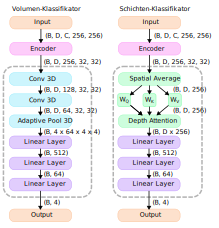
\includegraphics[width=0.9\linewidth]{Figures/Klassifikatoren.png}
  \caption{Architektur der beiden Klassifikatoren. Der Encoder wird jeweils modular ausgetauscht. 
  Links zu sehen ist die Architektur des \textit{Volumen-Klassifikators}, der die Merkmale, die der Encoder generiert, als Volumen interpretiert und mithilfe von 3D-Faltungen und Pooling daraus eine Repräsentation erzeugt.
  Diese Repräsentation wird anschließend durch Linear Layers in vier Ausgabe-Klassen umgeformt.
  Rechts ist der \textit{Schichten-Klassifikator} zu sehen.
  Die räumlichen X- und Y-Dimensionen werden im \textit{Schichten-Klassifikator} durch einen spatial average zusammengefasst.
  Durch eine Multihead Attention mit vier Attention-Köpfen und Embedding-Dimension 256 wird dann eine Repräsentation aus den individuellen Schichten der Merkmale erstellt.
  Lineare Layers formen anschließend die Repräsentation zu den vier Klassen um.}
  \label{fig:classifiers}
\end{figure}
\noindent
Der erste Klassifikator wird hier \textit{Volumen-Klassifikator} genannt.
Er interpretiert die Merkmale, die der Encoder generiert, als Volumen und generiert daraus mithilfe von 3D-Faltungen und Pooling eine neue Repräsentation.
Diese Repräsentation wird dann durch Linear Layers zu vier Ausgabe-Klassen umgeformt.
Die Idee des \textit{Volumen-Klassifikators} ist es, die Merkmale, die der Encoder generiert, möglichst vollständig zu erfassen und alle räumlichen Beziehungen, auch in Z-Richtung, festzustellen.
Hierbei ist das Ziel, dass durch die 3D-Faltungen eine domänenspezifische Interpretation der Merkmale gelernt wird, sodass die neuen Merkmale nach dem anschließenden Pooling aussagekräftig und niederdimensional sind.\\[0.5\baselineskip]
Außerdem wird hier der \textit{Schichten-Klassifikator} eingeführt.
Der \textit{Schichten-Klassifikator} betrachtet die einzelnen Schichten des Bilds anhand der individuellen Schichten, die der Encoder ausgibt, mithilfe eines Self-Attention-Mechanismus über die Z-Dimension. 
Dazu werden die räumlichen X- und Y-Dimensionen durch einen spatial average zusammengefasst.
Durch eine Multihead Attention mit vier Attention-Köpfen und Embedding-Dimension 256 wird eine Repräsentation aus den individuellen Schichten der Merkmale erstellt.
Lineare Layers formen anschließend die Repräsentation zu den vier Klassen um.
Für den \textit{Schichten-Klassifikator} ist das Ziel, dass durch die Vereinfachung der Daten aussagekräftige, schichtenweise Merkmale entstehen und dass diese räumlich invariant sind, da der betrachtete Nucleus in den Bildfenstern zentriert ist.
\newpage
\section{Segmentierung}
\subsection{Modelle}\label{sec:Seg_Modelle}
Für die Instanzsegmentierung der Nuclei werden die folgenden drei Modelle eingesetzt:
\begin{itemize}
  \item Ein Modell des nnU-Net Framework, das selbstkonfigurierte Modelle basierend auf der U-Net-Architektur erstellt \cite{isensee2021nnu}.
  \item Das DeepCell-Caliban-Modell, das Bildfaltungen und speziell entwickelten Nachverarbeitungsstrategien vereint.
  \item Cellpose-SAM, das die Architekturen der Cellpose-Modelle mit der Architektur und den Gewichten des Foundation-Model \ac{sam} vereint. 

\end{itemize}

\subsection{Nachverarbeitungsmethoden}\label{sec:Seg_PostProc}
Zur Nachbearbeitung der Instanzsegmentierungsmasken wird der Instanztrenner eingeführt.
Diese Methode dient dazu, separate Instanzen mit derselben numerischen Annotation (IDs) zu trennen und mit einzigartigen Zahlenwerten zu versehen. 
Pro Instanz werden hierzu ein zufälliges Pixel betrachtet und davon ausgehend alle Pixel mit direkter Verbindung über die Segmentierungsmaske gesucht.
Diese verbundenen Pixel werden als neue einzigartige Instanzen abgelegt, bis keine Pixel ohne Verbindung übrig bleiben. 
Eine weitere Methode der Nachbearbeitung, die auf Segmentierungsmasken eingesetzt werden kann, ist der Watershed-Algorithmus. %(siehe Abschnitt \ref{sec:Segmentierung}).
Der Algorithmus trennt überlagerte Instanzen, die das Modell als einzelne Instanzen segmentiert hat. 
%\begin{algorithm}
%\caption{Watershed-Nachbearbeitung zur Trennung überlappender Instanzen}\label{alg:watershed}
%\begin{algorithmic}
%\REQUIRE $maske_\text{instanz}$
%\ENSURE $maske_\text{refined}$
%
%\STATE $distanz \gets \text{DistanzTransformation}(maske_\text{instanz})$
%\STATE $marker \gets \text{LokaleMaxima}(distanz)$
%\STATE $gradient \gets -distance$
%\STATE $maske_\text{refined} \gets \text{Watershed}(gradient, marker)$
%
%\FOR{Region $r_i$ in $maske_\text{refined}$}
%  \IF{$Flaeche(r_i) < \tau$}
%    \IF{$r_i$ grenzt an größere Nachberregion $r_n$}
%      \STATE Vereinige $r_i$ mit $r_n$
%    \ELSE
%      \STATE Entferne $r_i$
%    \ENDIF
%  \ENDIF
%\ENDFOR
%
%\RETURN $maske_\text{refined}$
%\end{algorithmic}
%\end{algorithm}
